\section{Durchführung}
\label{sec:Durchführung}
In der Abbildung \ref{fig:aufbau} ist der Versuchsaufbau schematisch
dargestellt. Die Kupfer Probe ist von einem weitern Kuper zylinder
umschlossen und
befindet sich
in einem Rezipienten, der sich wiederum in einem
Dewargefäß befindet. Probe und Zylinder
sind jeweils mit einem Heizdraht umwickelt und können so
seperat von einander geheizt werden.
Die Temperatur an Probe und Zylinder wird jeweils über ein Ohmmeter
gemessen.
Um die Probe
zu kühlen, kann das Dewargefäß mit flüssigem Stickstoff
befüllt werden.
Zu Beginn der Messung wird die Probe auf $\SI{80}{\kelvin}$
heruntergekühlt.
Um diesen Vorgang zu beschleunigen wird in den Rezipienten Helium
gefüllt, um Konvektion zu förden. Bei einer Probentemperatur von $\SI{80}{\kelvin}$ wird das Helium aus dem
Rezipienten entfernt und ein
Vakuum im Rezipienten
erzeugt, damit die erhaltene Wärmemenge unabhängig von Konvektion wird.
Bei der eigentlichen Messung wird der Probe durch die Konstantstromquelle
Energie zugeführt und
in gleichen Zeitabständen $\delta t$
die Temperatur $T$ über das Ohmmeter gemessen.
Der Zylinder wird so aufgewärmt, dass
dieser stehts die gleiche Temperatur
besitzt wie die Probe.
Diese dient dazu Energieverlust
durch Wärmestrahlung der Probe zu minimieren.
Bei Abweichung der Temperatur muss der Heizstrom des Zylinder
nachgeregelt werden. Bei einer Temperatur von ungefähr $\SI{300}{\kelvin}$
ist die Messung abgeschlossen.


% Wärmeleitung Konvektion Wärmeabstrahlung

\begin{figure}
\centering
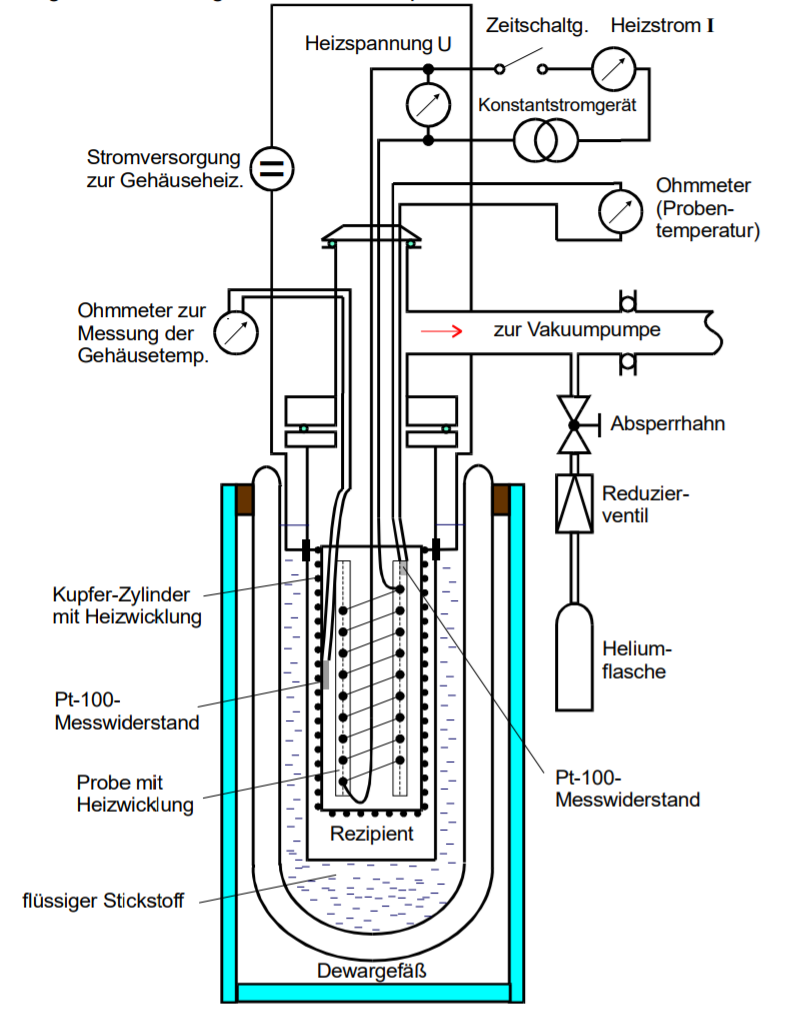
\includegraphics[width=0.7\textwidth]{Aufbau.PNG}
\caption{Schematischer Aufbau der Versuchsapparatur zur Bestimmung der Molwärme von Kupfer.}
\label{fig:aufbau}
\end{figure}
